%!TEX root = ../main.tex

\chapter{Introduction}\label{cha:introduction}

\section{Introduction}

There is this data that is pretty awesome, I'm going to plot it and show it to
you in sections~\ref{sec:the_data} and~\ref{sec:the_distribution_of_the_data}.


\section{The data}\label{sec:the_data}

In Figure~\ref{fig:the_data} we see data that was generated using
(\ref{equ:random_data}):

\begin{equation}
    x \in \{x \in \mathbb{Z}| 1 \leq x \leq 1999\}
\end{equation}

\begin{equation}
    y = 2(1 + \epsilon) x + 5\label{equ:random_data}
\end{equation}

where \(\epsilon\in(-0.5, 0.5)\) is a random number.

\begin{figure}[!hbtp]
    \begin{center}
        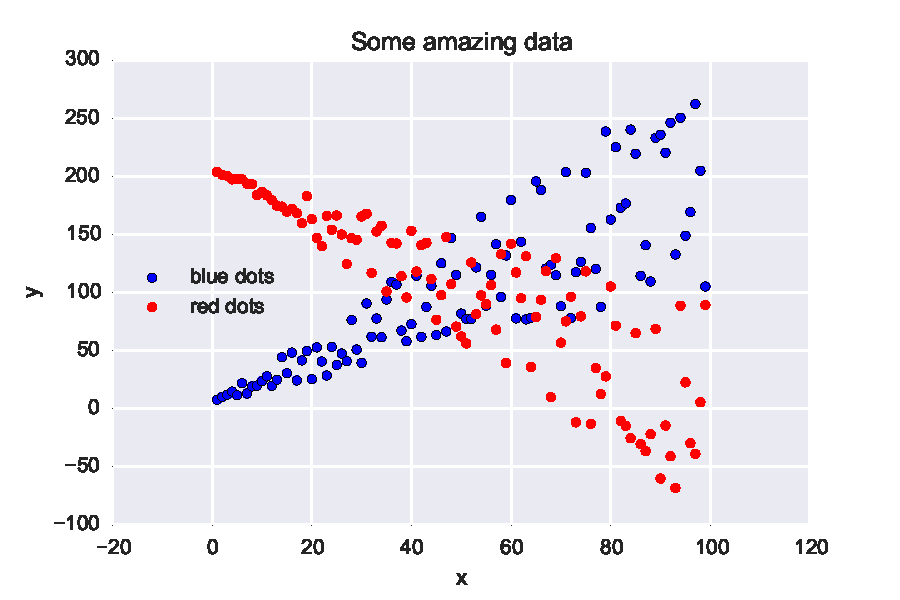
\includegraphics[width=.6\textwidth]{../img/plot1.pdf}
        \caption{The great data}\label{fig:the_data}
    \end{center}
\end{figure}

\section{The distribution of the data}\label{sec:the_distribution_of_the_data}

Figure shows the distribution of the data.

\begin{figure}[!hbtp]
    \begin{center}
        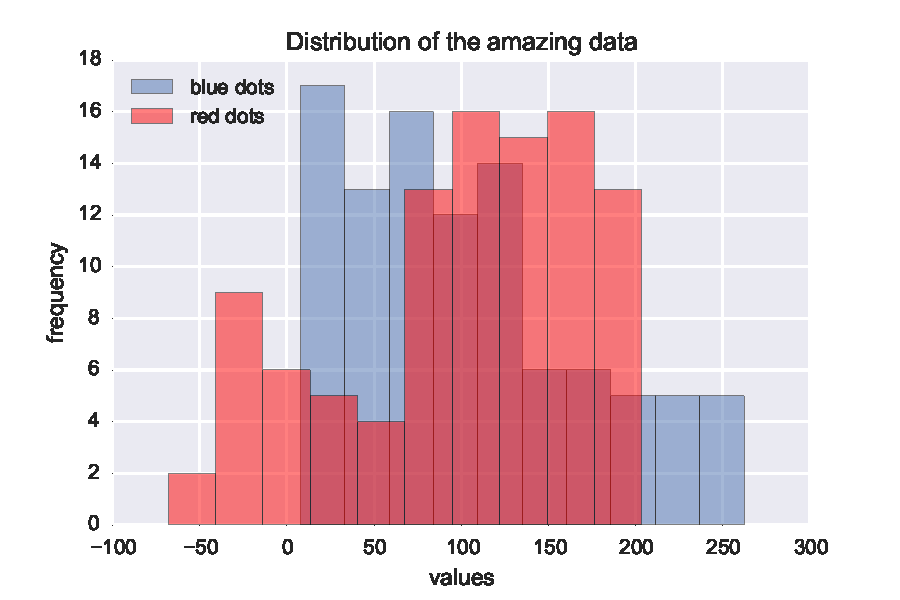
\includegraphics[width=.6\textwidth]{../img/plot2.pdf}
        \caption{The distribution of the great data}\label{fig:the_distribution_of_the_data}
    \end{center}
\end{figure}


%!TEX root = ../main.tex

\section{Conclusion}\label{sec:conclusion}

This chapter was amazing, here is a reference to a paper~\cite{Knight2016}.

